\section{Writing with Oggz\-Hungry callbacks}
\label{group__hungry}\index{Writing with OggzHungry callbacks@{Writing with OggzHungry callbacks}}
An Oggz\-Hungry callback will:\begin{itemize}
\item Create an {\em ogg\_\-packet\/} structure\item Add it to the packet queue with {\bf oggz\_\-write\_\-feed()}{\rm (p.\,\pageref{group__write__api_ga2})}\end{itemize}


Once you have set such a callback with {\bf oggz\_\-write\_\-set\_\-hungry\_\-callback()}{\rm (p.\,\pageref{group__write__api_ga1})}, simply call {\bf oggz\_\-write()}{\rm (p.\,\pageref{group__write__api_ga4})} or {\bf oggz\_\-write\_\-output()}{\rm (p.\,\pageref{group__write__api_ga3})} repeatedly, and OGGZ will call your callback to provide packets when it is hungry.

This process is illustrated in the following diagram:

\begin{figure}[H]
\begin{center}
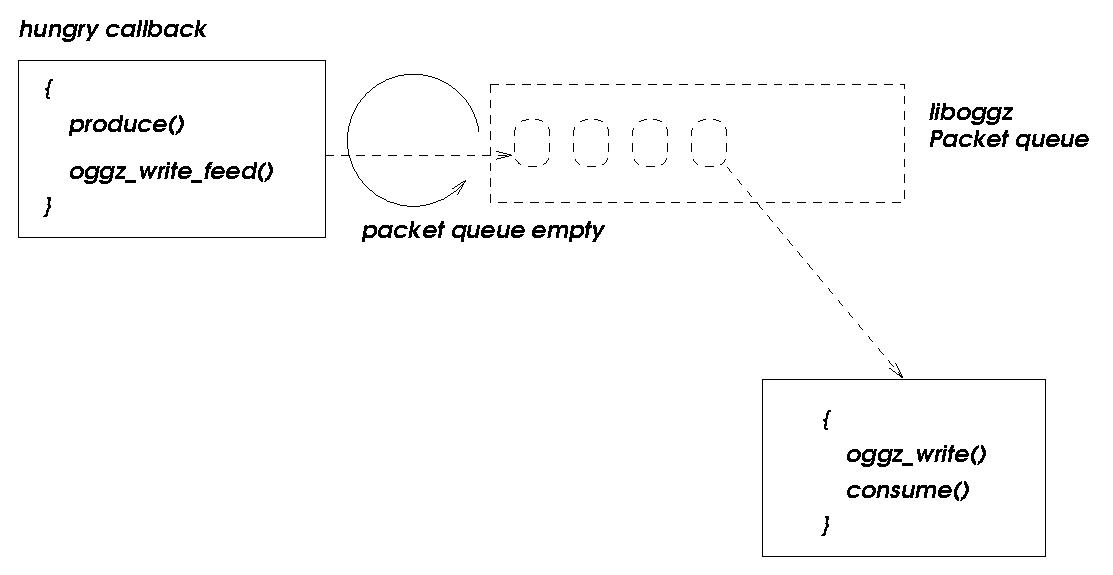
\includegraphics[width=10cm]{hungry}\caption{Using Oggz\-Hungry}
\end{center}
\end{figure}


The following example code generates a stream of ten packets, each containing a single byte ('A', 'B', ... , 'J'):



\footnotesize\begin{verbatim}
#include <stdlib.h> /* exit */
#include <oggz/oggz.h>

static long serialno;
static ogg_int64_t granulepos = 0;
static ogg_int64_t packetno = 0;

static int
hungry (OGGZ * oggz, int empty, void * user_data)
{
  ogg_packet op;
  unsigned char buf[1];

  buf[0] = 'A' + (int)packetno;

  op.packet = buf;
  op.bytes = 1;
  op.granulepos = granulepos;
  op.packetno = packetno;

  if (packetno == 0) op.b_o_s = 1;
  else op.b_o_s = 0;

  if (packetno == 9) op.e_o_s = 1;
  else op.e_o_s = 0;

  oggz_write_feed (oggz, &op, serialno, OGGZ_FLUSH_AFTER, NULL);

  granulepos += 100;
  packetno++;

  return 0;
}

int
main (int argc, char * argv[])
{
  char * progname, * filename = NULL;
  OGGZ * oggz;
  long n;

  progname = argv[0];
  if (argc > 1) filename = argv[1];

  if (filename) {
    oggz = oggz_open (filename, OGGZ_WRITE);
  } else {
    oggz = oggz_open_stdio (stdout, OGGZ_WRITE);
  }

  if (oggz == NULL) {
    fprintf (stderr, "%s: Error creating oggz\n", progname);
    exit (1);
  }

  serialno = oggz_serialno_new (oggz);

  if (oggz_write_set_hungry_callback (oggz, hungry, 1, NULL) == -1) {
    fprintf (stderr, "%s: Error setting OggzHungry callback\n", progname);
    exit (1);
  }

  while ((n = oggz_write (oggz, 32)) > 0);

  oggz_close (oggz);

  exit (0);
}
\end{verbatim}
\normalsize
 

